Der Simspark-Server kann verschiedene NAO-Modelle simulieren. Diese unterscheiden sich zum
Beispiel in der Länge der Extremitäten oder der Existenz von Zehen. Im Server-Verzeichnis
liegen eine Reihe von Ruby-Scene-Graph-Dateien, welche die geometrische Beschaffenheit der
verschiedenen Typen definieren. Konnektiert ein Bot auf den Server, so schickt dieser in seiner initialen Nachricht einen String mit, der auf das entsprechende Modell verweist.\\

Im Magma-Framework werden diese verschiedenen Modelle durch eigene AgentMetaModel[s]
abgebildet. Diese sind in eigenen Packages unter \texttt{magma.robots} organisiert. Initial waren im Framework fünf verschiedene Modelle enthalten ('nao', 'nao1', 'nao2', 'nao3' und 'naotoe').\\
Mit Hilfe des RunToPositionMetricBots (siehe: \ref{sse:Elem Bew:Laufen}) wurde das Modell 'nao', welches auf der Server-Datei: \textit{rsg/agent/nao/nao.rsg} basiert als bestes ausgewählt. Im Zuge der Laufoptimierung wurden sämtliche Parameter mit denen aus der Server-Konfiguration verglichen.
Aufgrund von Abweichungen wurde dann ein eigenes AgentMetaModel 'NaoRF' im Package
'robofreunde' erstellt, das diese behebt.\\
So wurden zum Beispiel die Translationsvektoren der Füße von \textit{'new Vector3D(0, 0.03, -0.035)'}
auf \textit{'new Vector3D(0, 0.03, -0.04)'} verlängert. (Entsprechend der \textit{setLocalPos}-Z-Komponente
\texttt{(def \$FootRelAnkle\_Z -0.04)} in \textit{data/rsg/agent/nao/naoleg.rsg})

\begin{figure}[H]
	\centering
	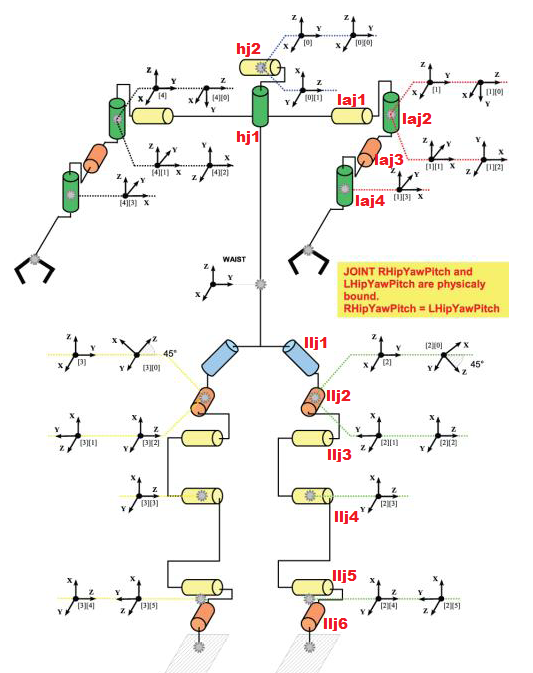
\includegraphics[width=240pt]{Grafiken/MetaModel/Nao_Body_Structure}
	\caption{Nao Meta Model}{Quelle: \texttt{https://en.wikipedia.org/wiki/File:Nao\_Body\_Structure\_\%28Labelled\%29.png}}
	\label{fig:dribblerekt}
\end{figure}

Die Auswahl der AgentMetaModel[s] erfolgt durch die zugehörige ComponentFactory (siehe: 
\ref{subsec:Agent Startup Routine} -factory). 